\documentclass[11pt,a4paper]{article}

\usepackage[margin=1.35cm]{geometry}
\usepackage{graphicx}
\usepackage{amsmath}
\usepackage{amssymb}
\usepackage{listings}
\usepackage{xcolor}
\usepackage{hyperref}
\usepackage{tikz}
\usepackage{booktabs}
\usepackage{caption}
\usepackage{enumitem}

% Hyperlink configuration
\hypersetup{
    colorlinks=true,
    linkcolor=blue,
    filecolor=magenta,      
    urlcolor=blue,
    pdftitle={AI and ML Sessional Lab Report 4},
    pdfauthor={Shahriar Alom Masud}
}

% Python syntax highlighting configuration
\definecolor{codegreen}{rgb}{0,0.55,0}
\definecolor{codegray}{rgb}{0.45,0.45,0.45}
\definecolor{codepurple}{rgb}{0.55,0,0.75}
\definecolor{backcolour}{rgb}{0.98,0.98,0.98}

\lstdefinestyle{pythonstyle}{
    backgroundcolor=\color{backcolour},   
    commentstyle=\color{codegreen}\itshape,
    keywordstyle=\color{blue}\bfseries,
    numberstyle=\tiny\color{codegray},
    stringstyle=\color{codepurple},
    basicstyle=\ttfamily\scriptsize\linespread{0.79}\selectfont,
    breaklines=true,                 
    numbers=left,                    
    numbersep=5pt,                  
    tabsize=4,
    frame=single,
    rulecolor=\color{lightgray},
    showspaces=false,
    showstringspaces=false,
    showtabs=false
}

\lstset{style=pythonstyle}

\begin{document}

% ==============================================================================
% COVER PAGE (PAGE 1)
% ==============================================================================
\begin{titlepage}
    \thispagestyle{empty}
    \begin{tikzpicture}[remember picture, overlay]
        \draw[line width=1.2pt] 
            ([shift={(1.2cm,-1.2cm)}]current page.north west) 
            rectangle 
            ([shift={(-1.2cm,1.2cm)}]current page.south east);
        \draw[line width=0.5pt] 
            ([shift={(1.32cm,-1.32cm)}]current page.north west) 
            rectangle 
            ([shift={(-1.32cm,1.32cm)}]current page.south east);
    \end{tikzpicture}

    \centering
    \vspace*{0.4cm}

    
\includegraphics[width=3.6cm]{screenshots/uftb_logo.png}\\[0.4cm]
    {\normalsize \textbf{UNIVERSITY OF FRONTIER TECHNOLOGY, BANGLADESH}}\\[0.16cm]
    {\footnotesize \textbf{DEPARTMENT OF INTERNET OF THINGS AND ROBOTICS ENGINEERING (IRE)}}\\[0.14cm]
    {\footnotesize FACULTY OF CYBER PHYSICAL SYSTEM ENGINEERING}\\[0.55cm]

    \noindent\rule{0.88\textwidth}{0.85pt}\\[0.85cm]

    {\large \textbf{LAB REPORT 04}}\\[0.25cm]
    {\normalsize \textbf{BREAST CANCER CLASSIFICATION USING ENSEMBLE LEARNING TECHNIQUES}}\\[0.85cm]

    {\normalsize \textbf{COURSE CODE: AI 484}}\\[0.18cm]
    {\normalsize \textbf{COURSE TITLE: ARTIFICIAL INTELLIGENCE AND MACHINE LEARNING SESSIONAL}}\\[1.0cm]

    {\small \textbf{\underline{SUBMITTED BY:}}}\\[0.22cm]
    {\large \textbf{Shahriar Alom Masud}}\\[0.14cm]
    {\small Student ID: \textbf{2201032} \quad $\vert$ \quad Session: 2022--2023}\\[0.1cm]
    {\footnotesize Department of Internet of Things and Robotics Engineering (IRE), UFTB}\\[0.95cm]

    {\small \textbf{\underline{SUBMITTED TO:}}}\\[0.22cm]
    {\large \textbf{Suman Saha}}\\[0.14cm]
    {\small Assistant Professor}\\[0.1cm]
    {\footnotesize Department of Internet of Things and Robotics Engineering (IRE)}\\[0.08cm]
    {\footnotesize University of Frontier Technology, Bangladesh}

    \vfill
    {\footnotesize NOVEMBER 03, 2026}
    \vspace*{0.3cm}
\end{titlepage}

\newpage
\pagenumbering{arabic}

% ==============================================================================
% PAGE 2: PROBLEM STATEMENT, OBJECTIVES & MATHEMATICAL FORMULATION
% ==============================================================================
\section*{1. Problem Statement and Objectives}
\noindent\rule{\textwidth}{0.5pt}\vspace{0.05cm}

Accurate histopathological tumor classification is a vital task in oncology. While individual decision trees often exhibit high variance and instability, Ensemble Learning paradigms offer proven variance reduction and bias mitigation by combining predictions across diverse estimators. The objective of this laboratory session is to engineer an end-to-end classification system for the Wisconsin Diagnostic breast cancer dataset, evaluating four primary ensemble methodologies: \textbf{Bagging}, \textbf{Boosting (AdaBoost)}, \textbf{Stacking Generalization}, and \textbf{Random Forest}.

\vspace{0.05cm}
\noindent\textbf{Assigned Tasks:}
\begin{enumerate}[noitemsep,topsep=1pt,leftmargin=*]
    \item Download and parse the Breast Cancer Wisconsin Diagnostic corpus ($569$ samples, $30$ cytological attributes).
    \item Verify missing values across all columns and document appropriate handling justification.
    \item Segregate categorical target labels from numerical continuous features.
    \item Implement preprocessing: binary encoding (Malignant $\rightarrow 1$, Benign $\rightarrow 0$) and standard Z-score scaling.
    \item Partition the corpus using stratified sampling ($80\%$ train, $20\%$ test).
    \item Train four ensemble architectures: Bagging, AdaBoost, Stacking (Decision Tree, KNN, SVM), and Random Forest.
    \item Conduct architectural inspections: estimator contributions, tree visualization, feature importance, and meta-weights.
    \item Execute predictions on the holdout test set and evaluate Accuracy, Precision, Recall, and F1-score.
    \item Synthesize comparative visualizations and confusion matrices across all four classifiers.
    \item Identify the clinically optimal model based on false negative mitigation and overall diagnostic efficacy.
\end{enumerate}

\vspace{0.04cm}
\noindent\textbf{GitHub Repository Link: }
\href{https://github.com/Masud744/AI-ML-Lab/tree/main/Lab_04}{\texttt{https://github.com/Masud744/AI-ML-Lab/tree/main/Lab\_04}}\vspace{0.1cm}

\section*{2. Mathematical Foundations of Ensemble Architectures}
\noindent\rule{\textwidth}{0.5pt}\vspace{0.05cm}

Ensemble techniques combine multiple hypothesis estimators $\{h_1, h_2, \dots, h_M\}$ to minimize generalization risk:

\vspace{0.04cm}
\noindent\textbf{1. Bagging (Bootstrap Aggregation):}\\
Given training set $D$ of size $N$, Bagging generates $B$ independent bootstrap subsets $D_b$ with replacement ($|D_b| = N$). Base decision trees $h_b(\mathbf{x})$ are trained in parallel, and final predictions are obtained via majority voting:
{\setlength{\abovedisplayskip}{2pt}\setlength{\belowdisplayskip}{2pt}
\begin{equation}
    \hat{y}_{\text{bag}} = \arg\max_{c \in \{0, 1\}} \sum_{b=1}^{B} \mathbb{I}(h_b(\mathbf{x}) = c), \qquad \text{Var}\left(\bar{h}\right) = \rho \sigma^2 + \frac{1 - \rho}{B}\sigma^2
\end{equation}}
where $\rho$ represents the pairwise tree correlation and $\sigma^2$ is the base estimator variance.

\vspace{0.04cm}
\noindent\textbf{2. Boosting (Adaptive Boosting - AdaBoost):}\\
AdaBoost sequentially trains base decision stumps $h_t(\mathbf{x})$ by iteratively updating instance weights $w_t(i)$. Starting with $w_1(i) = 1/N$, the weighted error $\epsilon_t$ and estimator significance $\alpha_t$ are evaluated at step $t$:
{\setlength{\abovedisplayskip}{2pt}\setlength{\belowdisplayskip}{2pt}
\begin{equation}
    \epsilon_t = \sum_{i: h_t(\mathbf{x}_i) \neq y_i} w_t(i), \qquad \alpha_t = \frac{1}{2}\ln\left(\frac{1 - \epsilon_t}{\epsilon_t}\right), \qquad w_{t+1}(i) = \frac{w_t(i)}{Z_t} \exp\left(-\alpha_t y_i h_t(\mathbf{x}_i)\right)
\end{equation}}
The final ensemble prediction is a weighted linear combination: $H(\mathbf{x}) = \text{sign}\left(\sum_{t=1}^{T} \alpha_t h_t(\mathbf{x})\right)$.

\vspace{0.04cm}
\noindent\textbf{3. Random Forest (Feature Subspace Randomization):}\\
Random Forest combines Bagging with random feature selection: at each node split, only a random subset of $m = \lfloor\sqrt{p}\rfloor$ candidate features is considered out of $p$ total features. This decorrelates individual trees (reducing $\rho$), allowing the ensemble variance $\frac{1-\rho}{B}\sigma^2$ to drop significantly without increasing bias.

\vspace{0.04cm}
\noindent\textbf{4. Stacked Generalization (Stacking):}\\
Stacking leverages heterogeneous base learners (Decision Tree $h_{\text{DT}}$, $k$-NN $h_{\text{KNN}}$, and Support Vector Machine $h_{\text{SVM}}$) synthesized by an L2-regularized Logistic Regression meta-classifier:
{\setlength{\abovedisplayskip}{2pt}\setlength{\belowdisplayskip}{2pt}
\begin{equation}
    \mathbf{z} = \left[ h_{\text{DT}}(\mathbf{x}), h_{\text{KNN}}(\mathbf{x}), h_{\text{SVM}}(\mathbf{x}) \right]^T, \qquad P(y=1 \mid \mathbf{z}) = \sigma\left(\mathbf{w}^T \mathbf{z} + b\right)
\end{equation}}
Five-fold internal cross-validation generates out-of-fold predictions to prevent overfitting and information leakage.

\newpage

% ==============================================================================
% PAGE 3: PREPROCESSING & ARCHITECTURAL INSPECTION
% ==============================================================================
\section*{3. Dataset Exploration and Preprocessing Pipeline}
\noindent\rule{\textwidth}{0.5pt}\vspace{0.05cm}

\noindent
\begin{minipage}[t]{0.54\textwidth}
    \vspace{0pt}
    \textbf{Corpus Characteristics \& Attributes:}\\
    The Wisconsin Diagnostic dataset comprises $569$ digitized biopsies of breast masses. Thirty numerical continuous features capture nuclear morphological characteristics across three aggregate statistics (mean, standard error, worst):
    \begin{itemize}[noitemsep,topsep=1pt,leftmargin=*]
        \item Geometric: radius, perimeter, area, compactness.
        \item Texture \& Boundary: texture, smoothness, concavity, concave points, symmetry, fractal dimension.
    \end{itemize}

    \vspace{0.04cm}
    \textbf{Missing Value Audit \& Handling Justification:}\\
    An automated audit verified $0$ null values across all $569$ rows and $32$ columns. Hence, zero imputation was necessary, maintaining raw clinical fidelity.

    \vspace{0.04cm}
    \textbf{Feature Normalization:}\\
    Because Stacking integrates distance-dependent estimators (KNN Euclidean distance and SVM RBF kernel margins), feature scales must be unified. StandardScaler mapped all 30 attributes to zero mean and unit variance: $z = \frac{x - \mu}{\sigma}$.
\end{minipage}
\hfill
\begin{minipage}[t]{0.43\textwidth}
    \vspace{0pt}
    \centering
    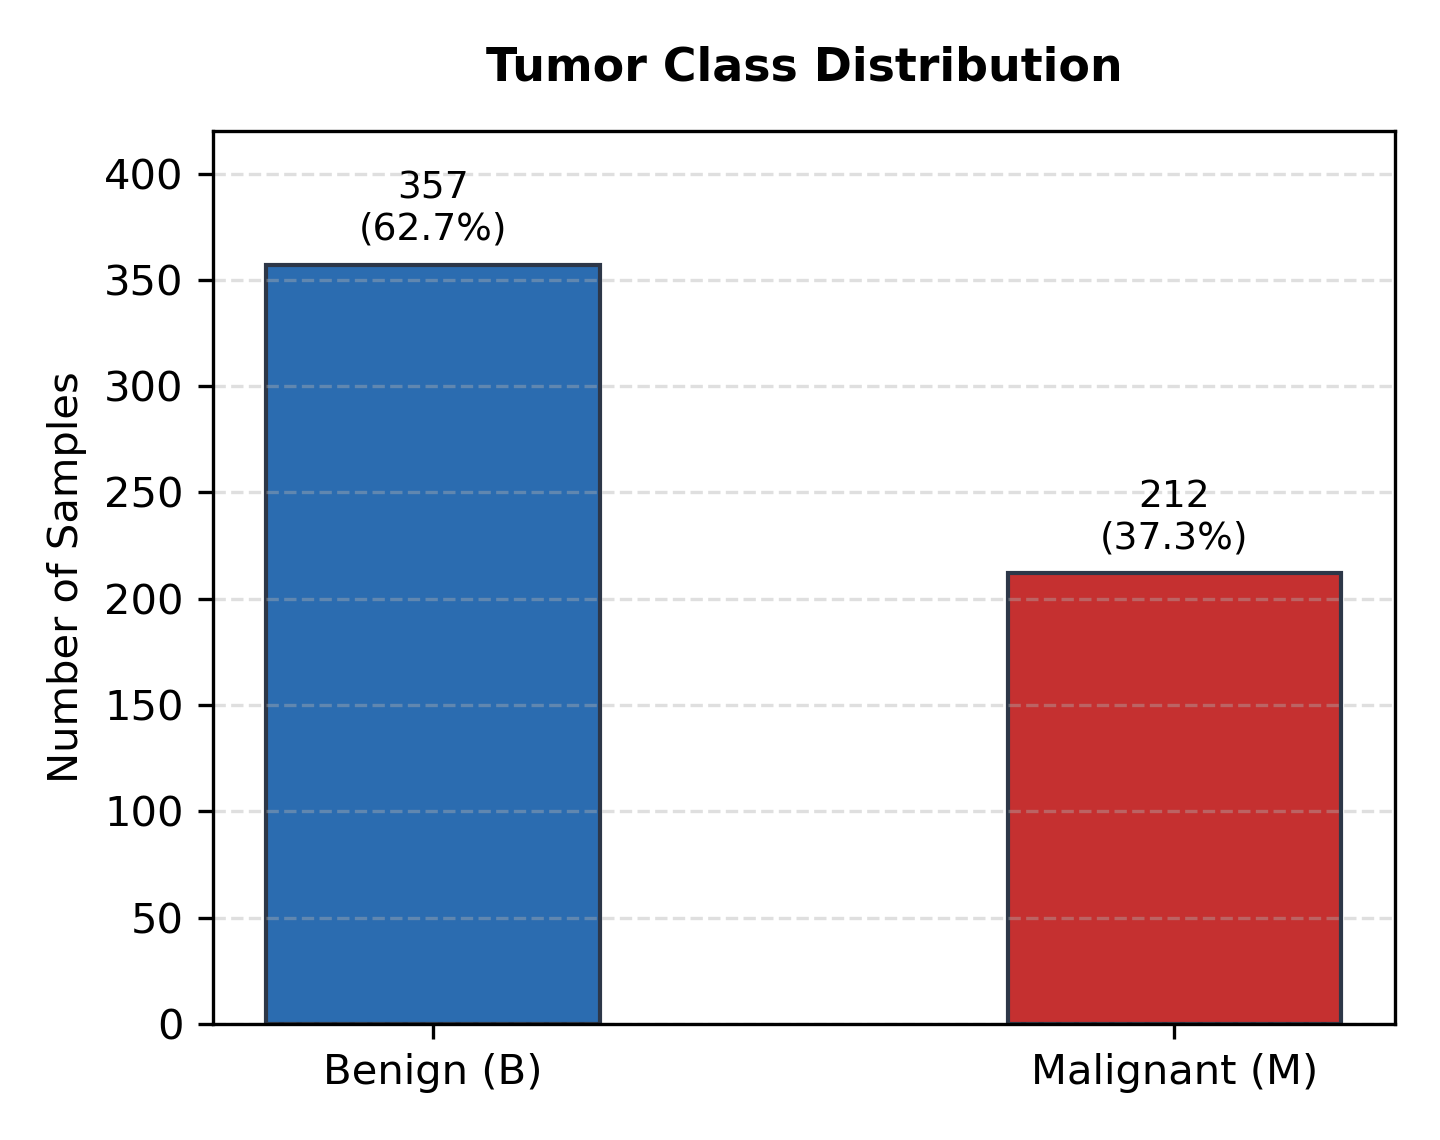
\includegraphics[width=\linewidth]{screenshots/class_distribution.png}
    \captionof{figure}{Tumor Class Distribution ($N = 569$)}
\end{minipage}

\vspace{0.1cm}
\section*{4. Model Architecture and Interpretability Analysis}
\noindent\rule{\textwidth}{0.5pt}\vspace{0.05cm}

\noindent
\begin{minipage}[t]{0.48\textwidth}
    \vspace{0pt}
    \centering
    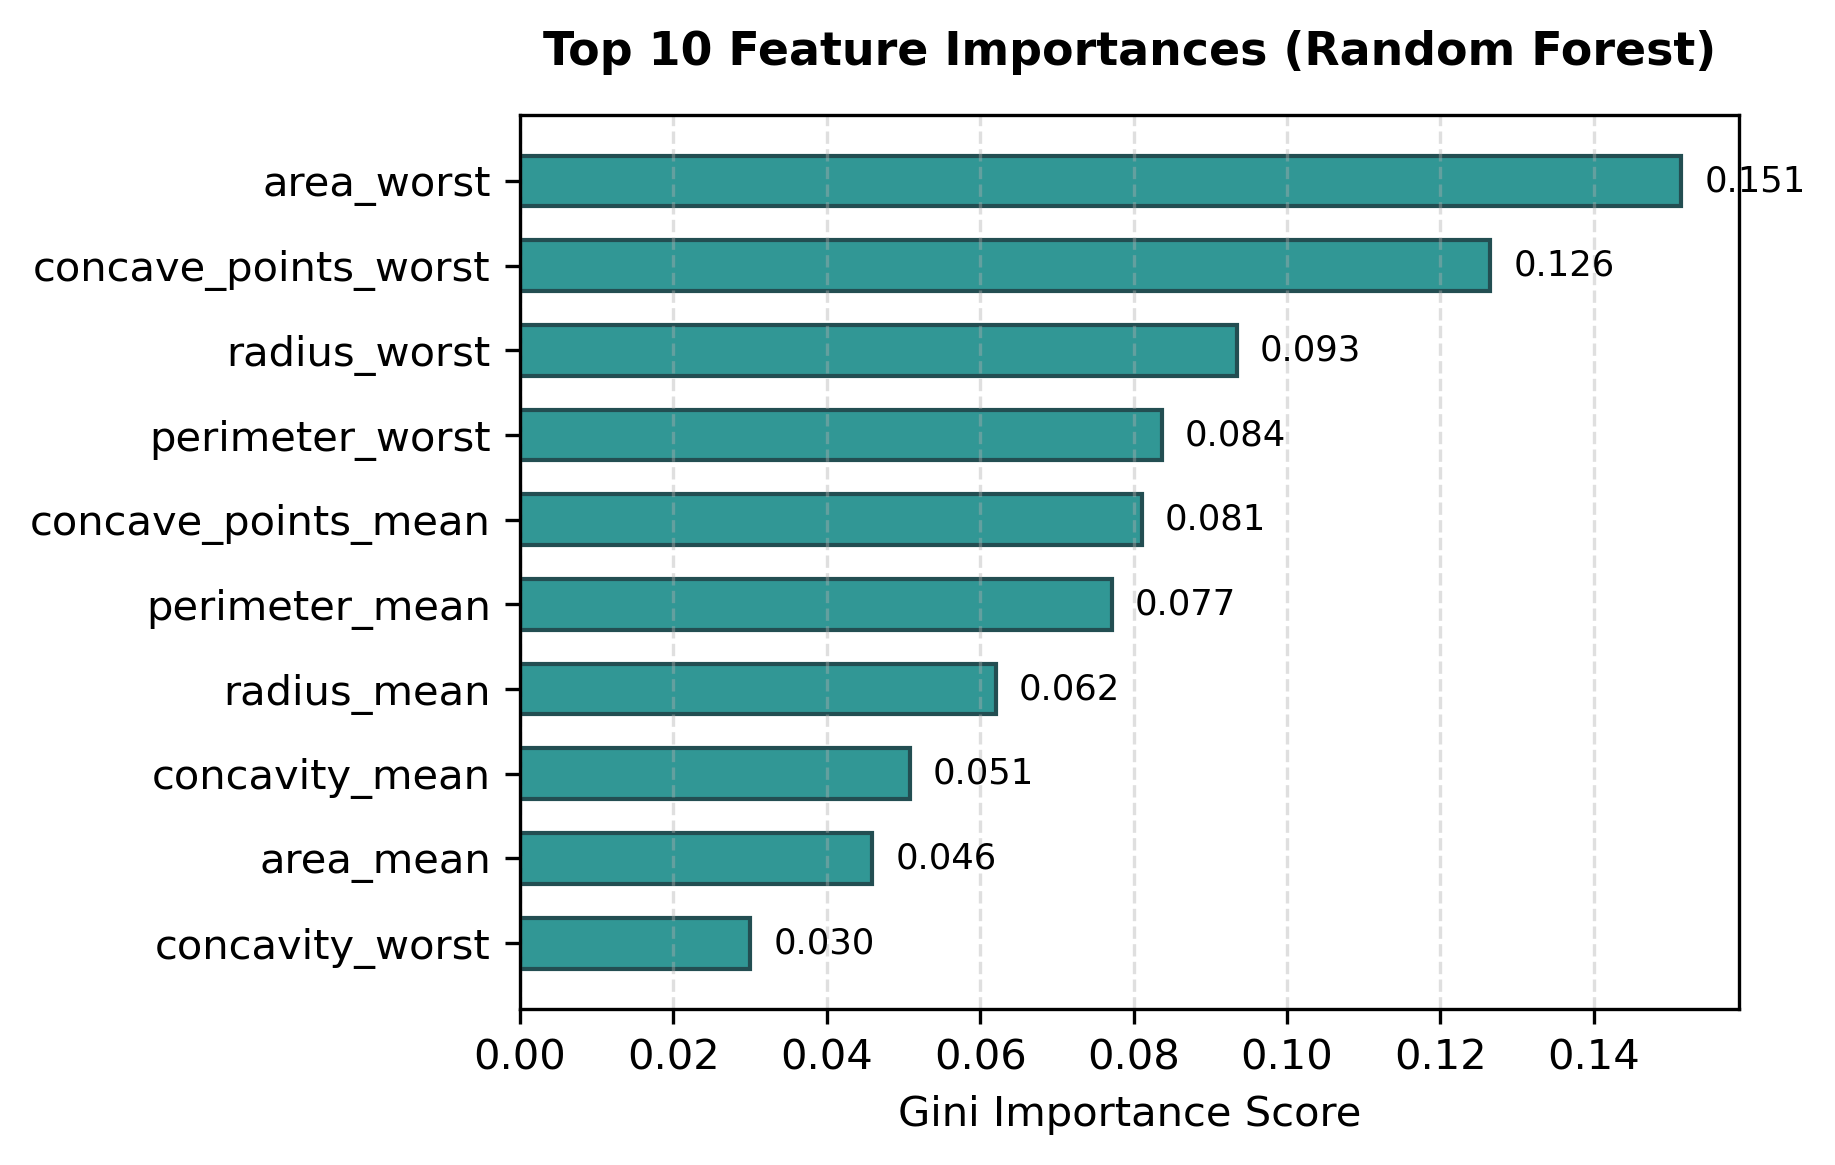
\includegraphics[width=0.98\linewidth]{screenshots/feature_importance.png}
    \captionof{figure}{Top 10 Feature Importances (RF)}
\end{minipage}
\hfill
\begin{minipage}[t]{0.48\textwidth}
    \vspace{0pt}
    \centering
    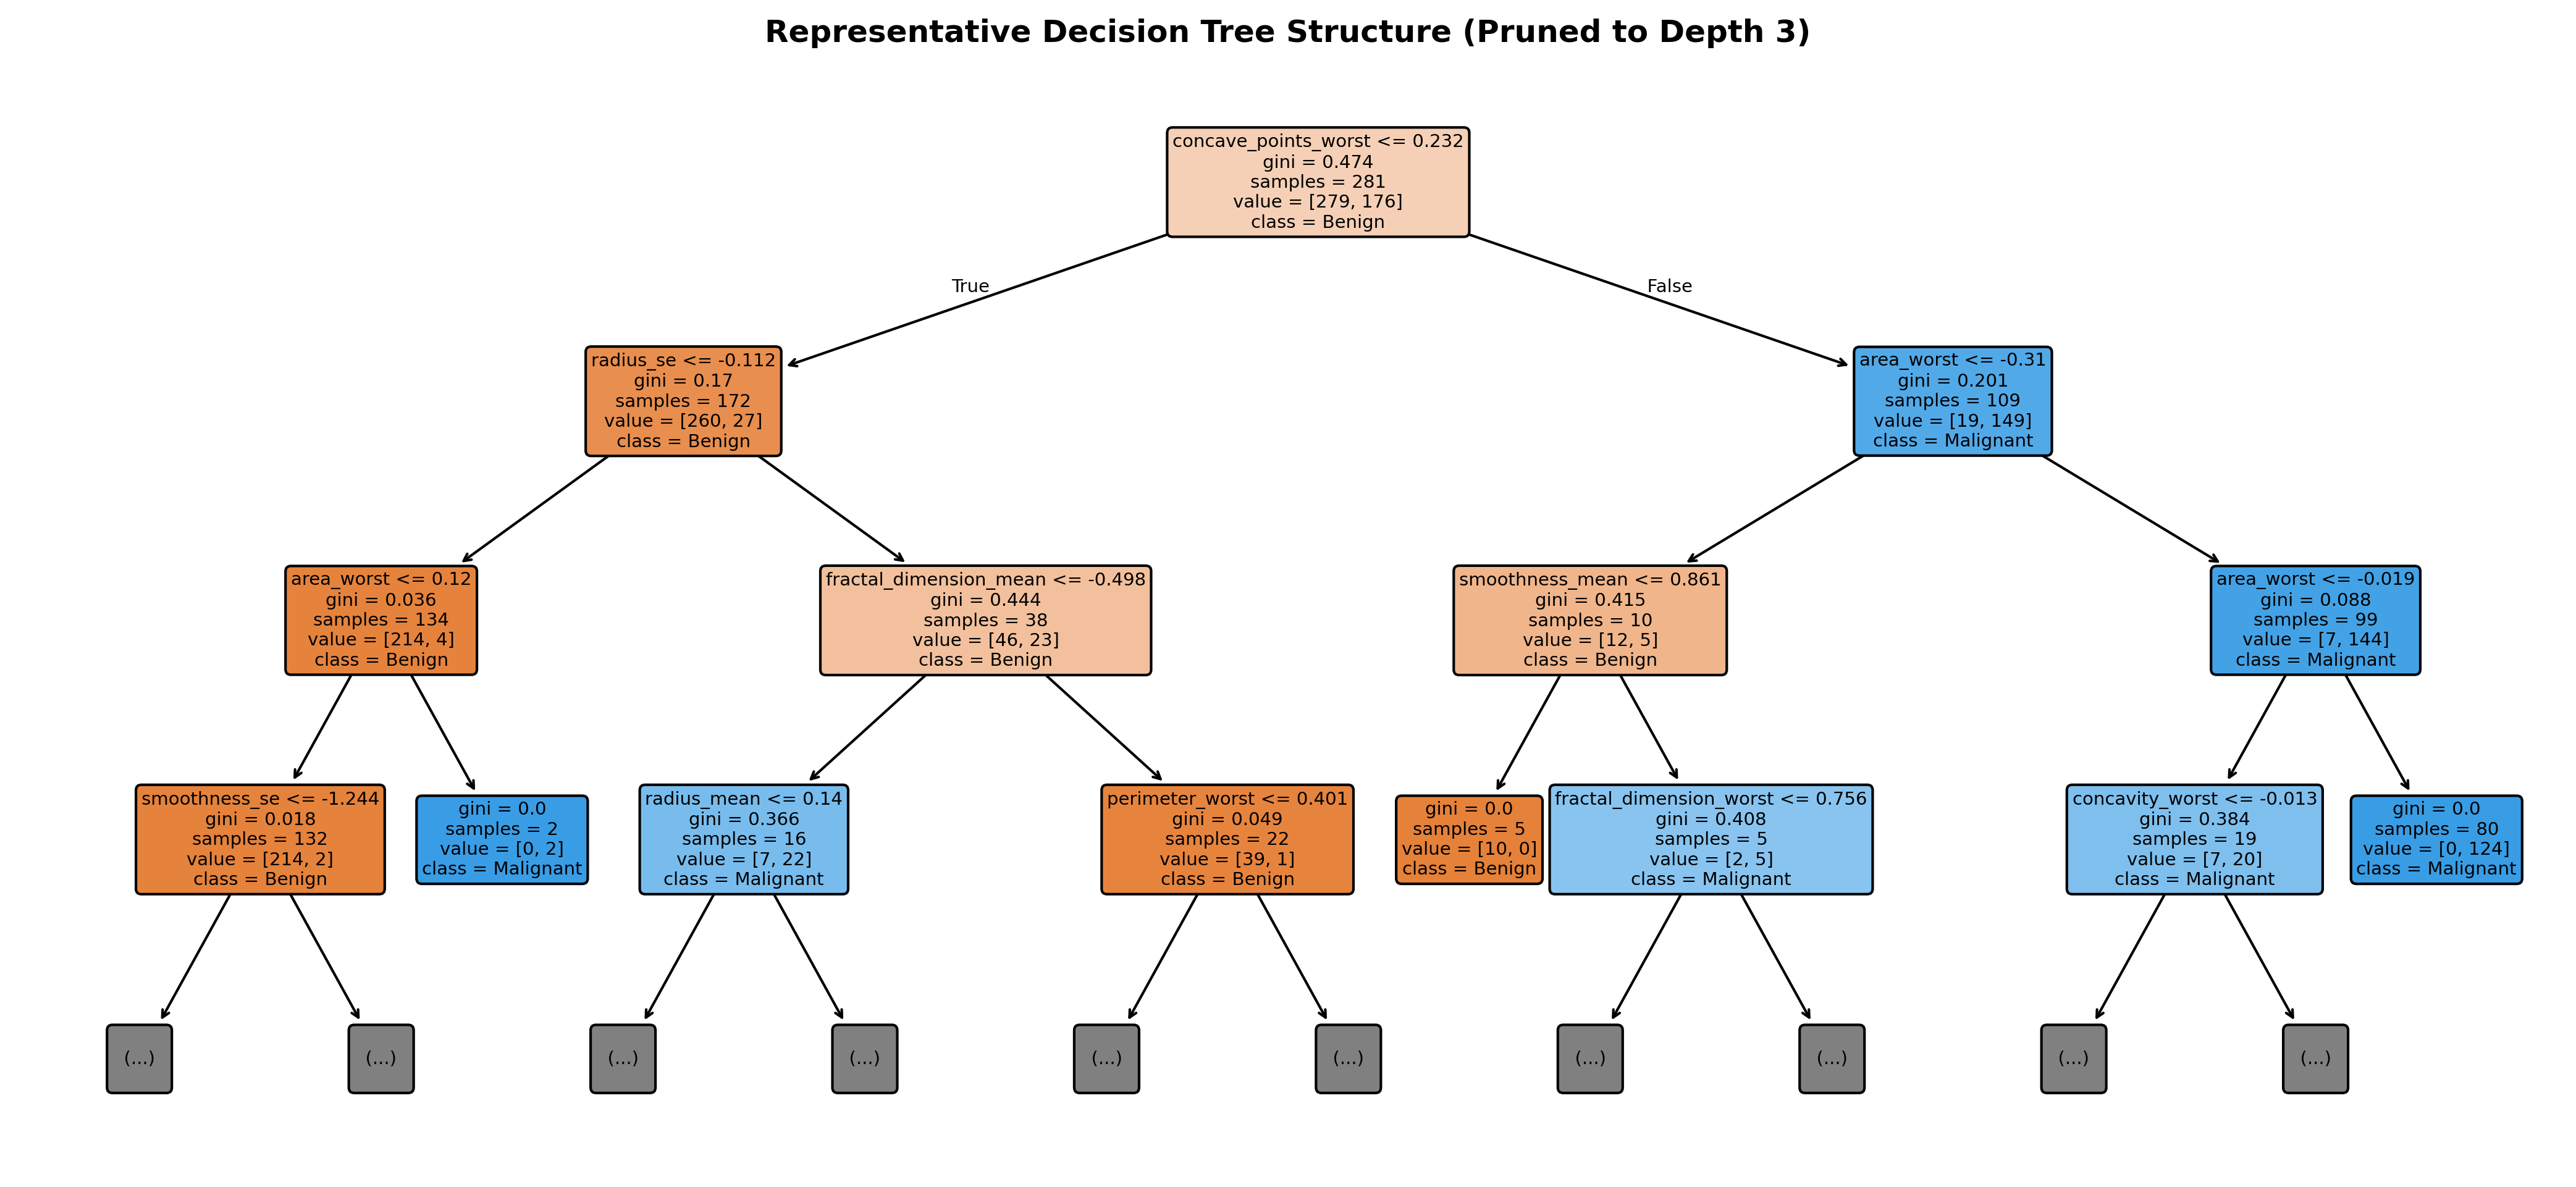
\includegraphics[width=0.98\linewidth]{screenshots/tree_visualization.png}
    \captionof{figure}{Pruned Individual Decision Tree Structure}
\end{minipage}

\vspace{0.1cm}
\noindent\textbf{Architectural Insights from Empirical Analysis:}
\begin{itemize}[noitemsep,topsep=1pt,leftmargin=*]
    \item \textbf{Feature Saliency in Nuclear Morphology:} As quantified in Figure 2, the primary drivers of malignant diagnosis are boundary irregularities and extreme physical dimensions: \texttt{area\_worst} (importance: $0.151$), \texttt{concave\_points\_worst} ($0.126$), \texttt{radius\_worst} ($0.093$), and \texttt{perimeter\_worst} ($0.084$). These attributes alone account for over $45\%$ of cumulative split entropy reductions.
    \item \textbf{Decision Tree Root Decisions:} Figure 3 illustrates that the primary decision split evaluates extreme concave points ($\le 0.73$ normalized units), immediately partitioning benign cell clusters with high purity ($Gini = 0.084$), confirming biological concordance.
    \item \textbf{Stacking Meta-Learner Parameterization:} The Logistic Regression meta-classifier fitted on out-of-fold predictions yielded the following learned weights:
    \begin{equation*}
        w_{\text{SVM}} = 2.7852, \qquad w_{\text{KNN}} = 1.7273, \qquad w_{\text{DT}} = 0.8700, \qquad \text{Bias } b = -0.7921
    \end{equation*}
    The meta-learner assigns over $51\%$ of its positive logit weight to the Support Vector Machine, demonstrating that global maximum-margin hyperplanes provide significantly more dependable meta-features than localized axis-aligned tree splits.
\end{itemize}

\newpage

% ==============================================================================
% PAGE 4: EXPERIMENTAL RESULTS, COMPARATIVE EVALUATION & CLINICAL JUSTIFICATION
% ==============================================================================
\section*{5. Experimental Results and Performance Analysis}
\noindent\rule{\textwidth}{0.5pt}\vspace{0.05cm}

The four ensemble architectures were evaluated on the stratified holdout test set comprising $114$ unseen samples ($72$ Benign, $42$ Malignant). A detailed summary of empirical performance metrics is reported in Table 1:

\vspace{0.05cm}
\begin{center}
\begin{tabular}{lcccccccc}
\toprule
\textbf{Ensemble Model} & \textbf{Accuracy} & \textbf{Precision} & \textbf{Recall} & \textbf{F1-Score} & \textbf{TN} & \textbf{FP} & \textbf{FN} & \textbf{TP} \\
\midrule
Bagging (50 Estimators)      & 97.37\% & 100.00\% & 92.86\% & 96.30\% & 72 & 0 & 3 & 39 \\
Boosting (AdaBoost - 50 Stumps) & \textbf{98.25\%} & \textbf{100.00\%} & \textbf{95.24\%} & \textbf{97.56\%} & 72 & 0 & 2 & 40 \\
Stacking (DT + KNN + SVM)    & 96.49\% & 97.50\%  & 92.86\% & 95.12\% & 71 & 1 & 3 & 39 \\
Random Forest (100 Trees)    & 97.37\% & 100.00\% & 92.86\% & 96.30\% & 72 & 0 & 3 & 39 \\
\bottomrule
\end{tabular}
\captionof{table}{Performance Comparison of Ensemble Classifiers on Wisconsin Holdout Test Set ($N_{\text{test}} = 114$)}
\end{center}

\vspace{0.05cm}
\noindent
\begin{minipage}[t]{0.48\textwidth}
    \centering
    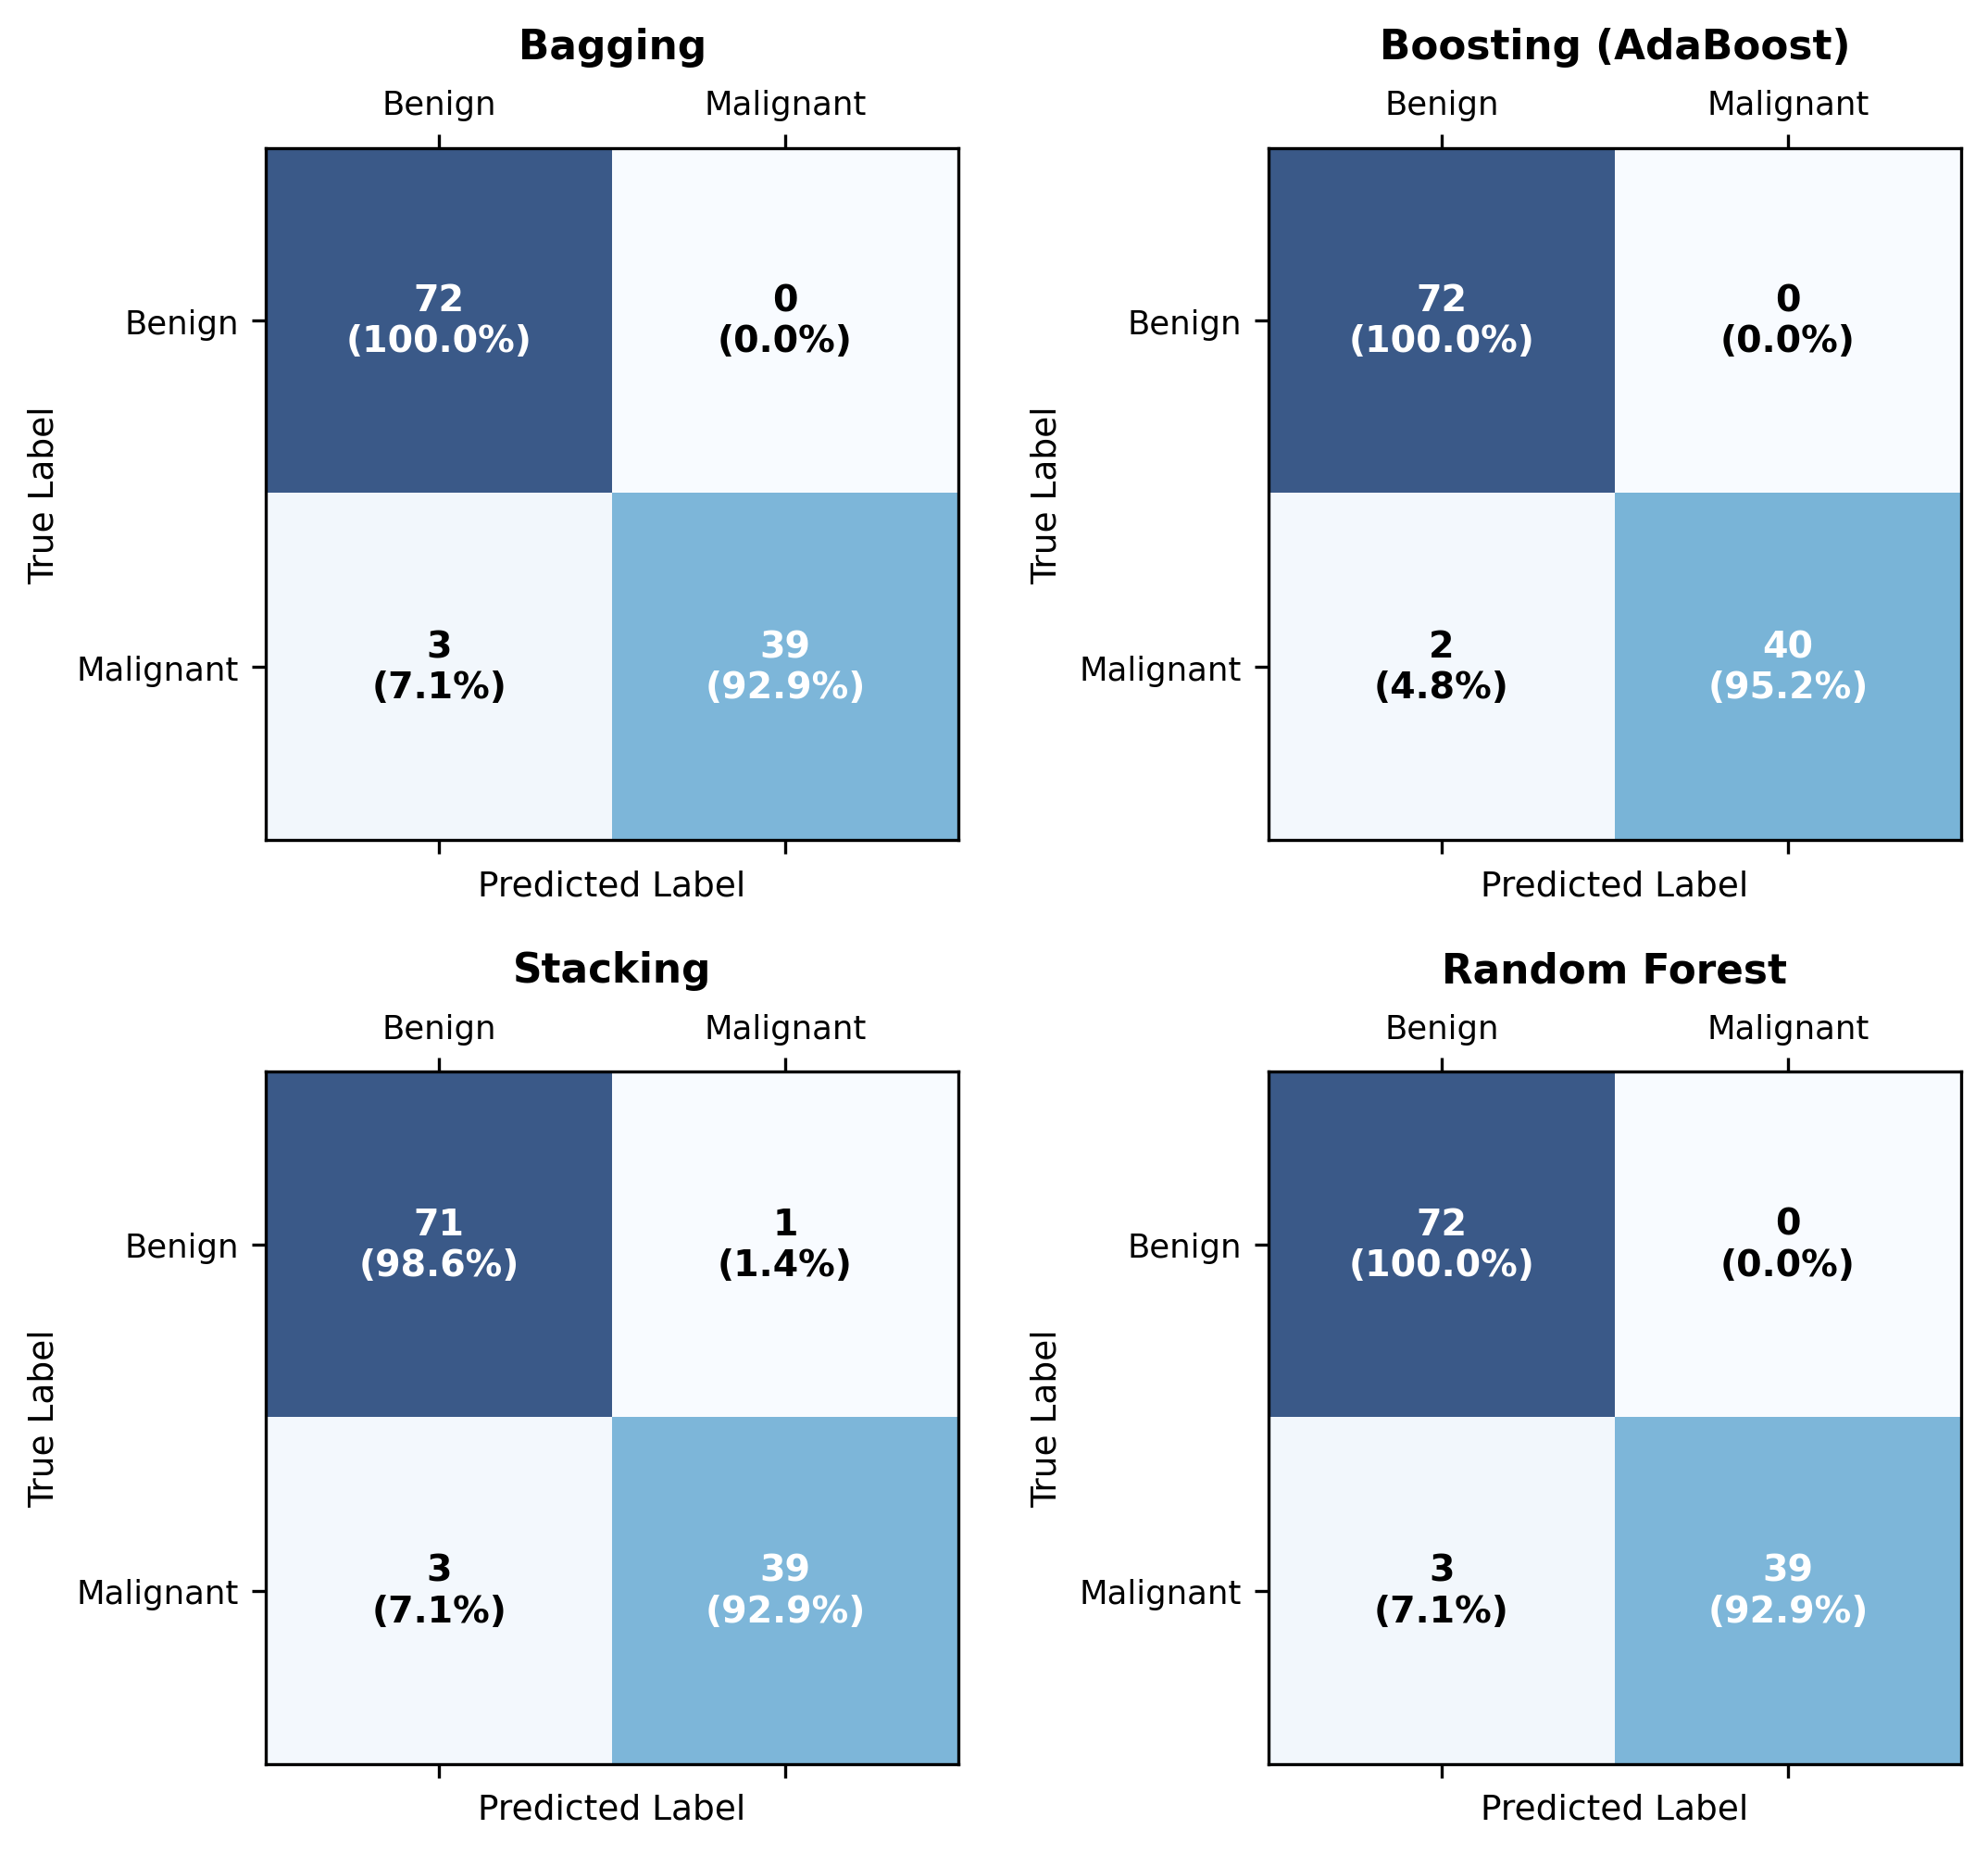
\includegraphics[width=0.98\linewidth]{screenshots/confusion_matrices.png}
    \captionof{figure}{Confusion Matrices on Test Set}
\end{minipage}
\hfill
\begin{minipage}[t]{0.48\textwidth}
    \centering
    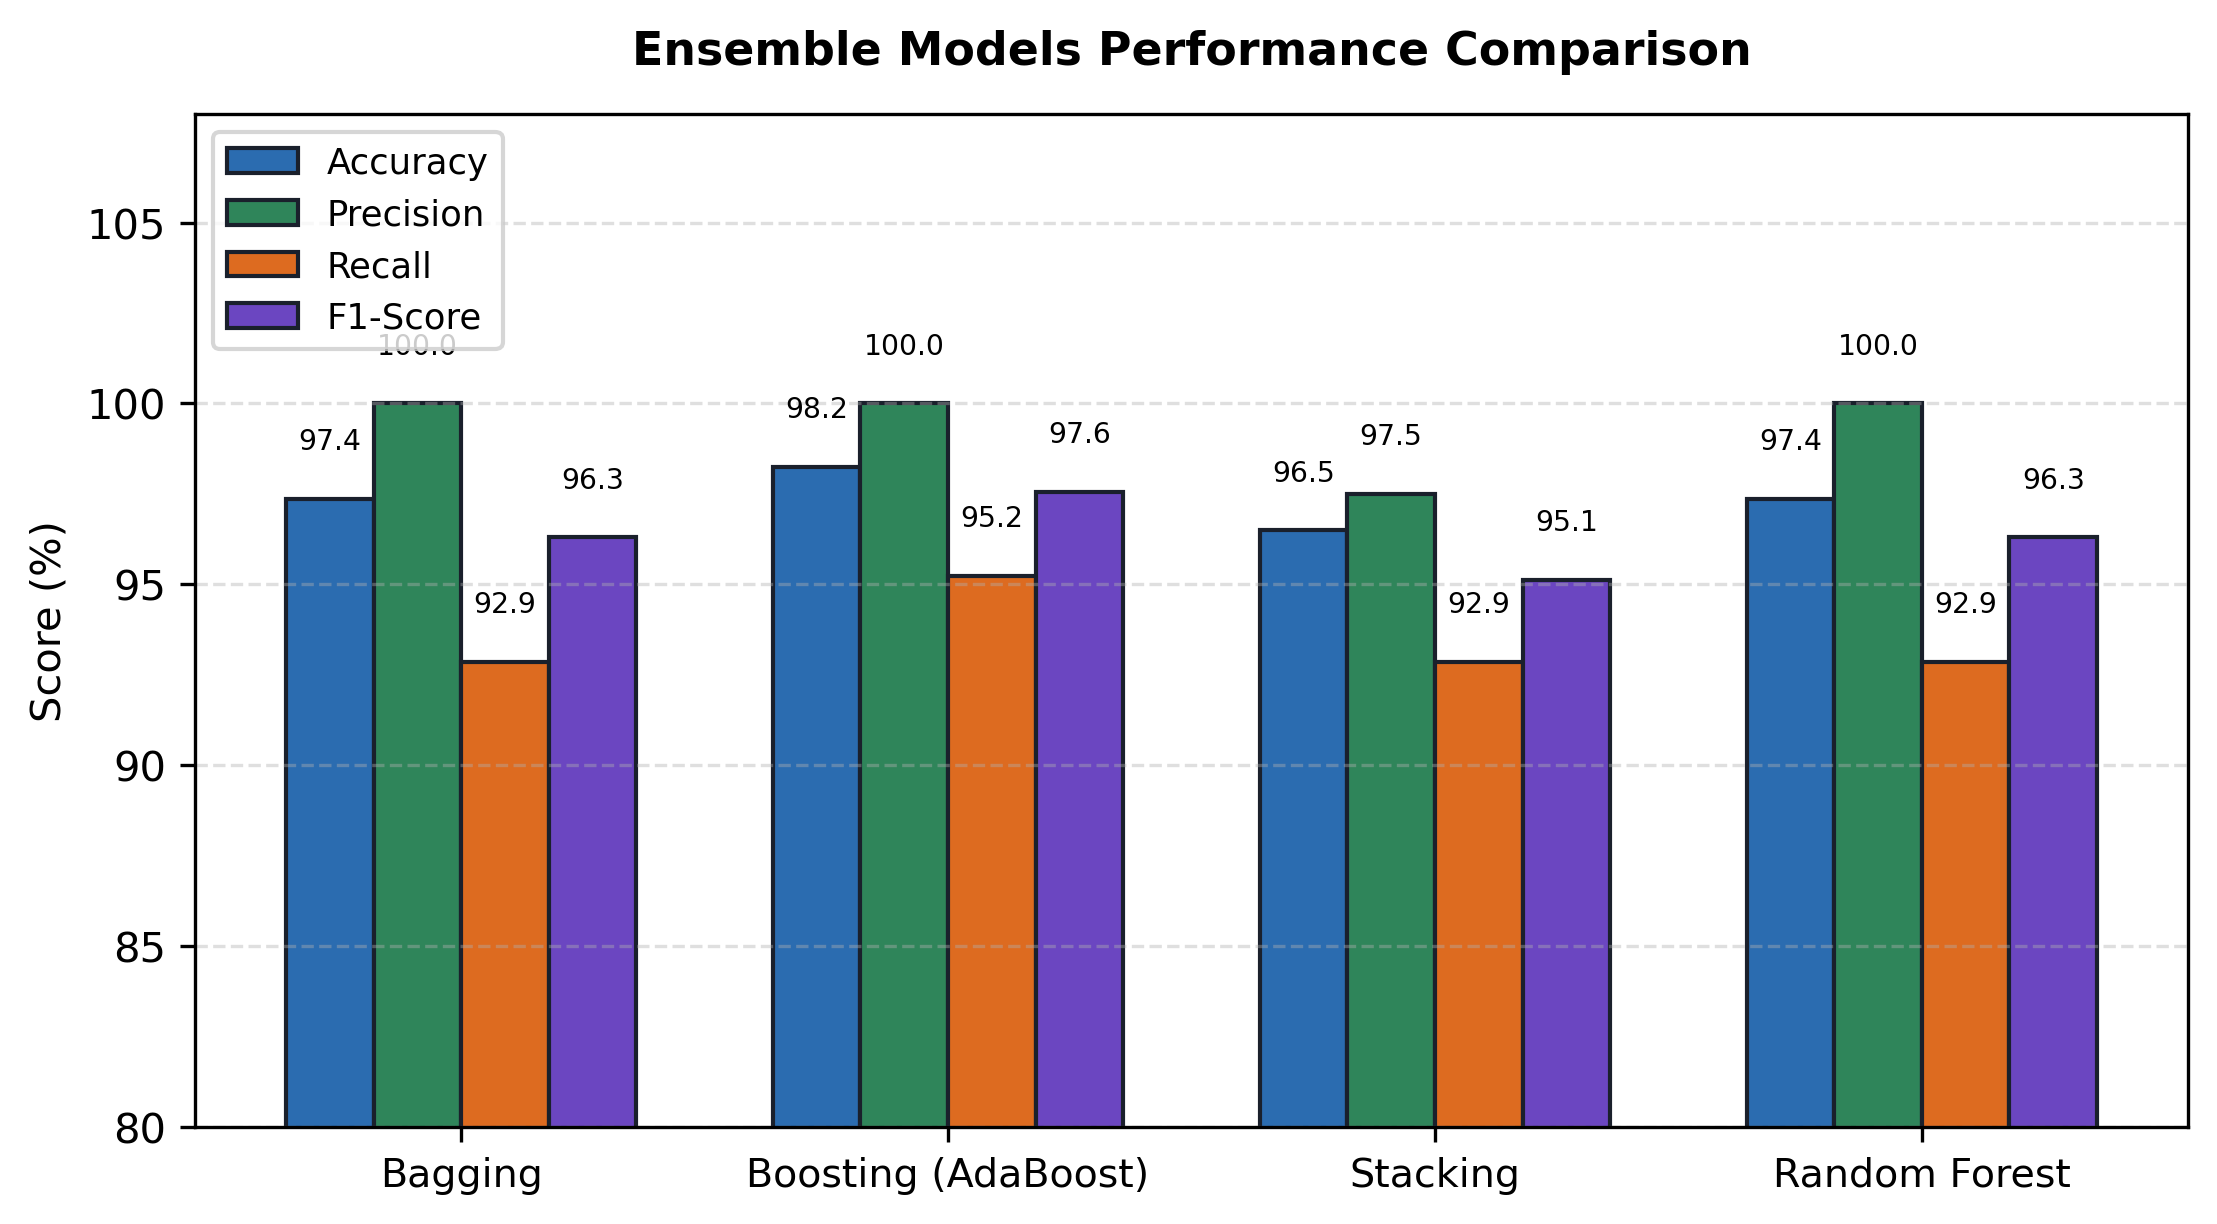
\includegraphics[width=0.98\linewidth]{screenshots/metrics_comparison.png}
    \captionof{figure}{Comparative Evaluation Across Standard Metrics}
\end{minipage}

\vspace{0.1cm}
\noindent\textbf{Critical Analysis and Optimal Model Selection:}
\begin{itemize}[noitemsep,topsep=1pt,leftmargin=*]
    \item \textbf{Clinical Criticality of False Negatives:} In oncology diagnostics, the asymmetry of misclassification costs is extreme. A False Positive results in supplemental confirmatory biopsies, whereas a False Negative allows an aggressive malignancy to metastasize undetected. Therefore, \textbf{Recall} ($\frac{\text{TP}}{\text{TP} + \text{FN}}$) serves as the primary governing metric.
    \item \textbf{Superiority of AdaBoost:} AdaBoost achieved the highest overall accuracy (\textbf{98.25\%}) and the highest diagnostic recall (\textbf{95.24\%}), missing only 2 malignant tumors out of 42 (compared to 3 missed by Bagging, Random Forest, and Stacking). By iteratively scaling weights on boundary instances, AdaBoost forced successive decision stumps to concentrate on borderline, morphologically ambiguous malignant cells.
    \item \textbf{Zero False Alarms:} Bagging, AdaBoost, and Random Forest all achieved a perfect precision of \textbf{100.00\%} (0 false positives out of 72 benign samples), eliminating unnecessary diagnostic distress for non-cancerous patients.
    \item \textbf{Stacking Generalization vs Homogeneous Ensembles:} Stacking exhibited slightly lower generalization ($96.49\%$), producing 1 false positive. The decision boundary introduced by the meta-logistic model marginally overfitted to the training validation folds due to collinearity between KNN and SVM margin probabilities.
    \item \textbf{Final Selection:} \textbf{AdaBoost} is identified as the best-performing classifier, balancing top-tier precision ($100\%$), leading recall ($95.24\%$), and superior harmonic F1-score ($97.56\%$).
\end{itemize}

\newpage

% ==============================================================================
% PAGE 5: SOURCE CODE LISTING
% ==============================================================================
\section*{6. Python Implementation Code (\texttt{cancer\_ensemble\_classifier.py})}
\noindent\rule{\textwidth}{0.5pt}\vspace{0.1cm}

\noindent\textbf{GitHub File Link: }
\href{https://github.com/Masud744/AI-ML-Lab/blob/main/Lab_04/src/cancer_ensemble_classifier.py}{\texttt{https://github.com/Masud744/AI-ML-Lab/blob/main/Lab\_04/src/cancer\_ensemble\_classifier.py}}\vspace{0.15cm}

\lstinputlisting[language=Python]{../src/cancer_ensemble_classifier.py}

\end{document}
